\documentclass[a0paper, portrait]{tikzposter}

% --- PAKIETY ---
\usepackage[utf8]{inputenc}
\usepackage[T1]{fontenc}
\usepackage{polski}
\usepackage{amsfonts, amsmath, amssymb}
\usepackage{graphicx}

% --- KOLORY PWR ---
\definecolor{PWrRed}{HTML}{AA151B}
\definecolor{PWrGrey}{HTML}{333333}

% --- STYLIZACJA ---
\usetheme{Default}
\useblockstyle[bodyinnersep=0.4cm, titleinnersep=0.2cm]{Minimal}
\colorlet{backgroundcolor}{white}
\colorlet{blocktitlefgcolor}{PWrRed}
\colorlet{blocktitlebgcolor}{white}
\usetitlestyle{Empty} 

% --- NAGŁÓWEK ---
\settitle{
    \begin{minipage}{\textwidth}
        \begin{minipage}{0.12\textwidth}
            \raggedright 
            
\includegraphics[width=0.6\linewidth]{logo_pwr.jpg}
        \end{minipage}
        \begin{minipage}{0.85\textwidth}
            \raggedright
            \color{PWrGrey}
            {\fontsize{64}{72} \selectfont \bfseries Parliamentary Network Analysis using Sejm RP API \par}
            \vspace{0.4cm}
            {\fontsize{36}{42} \selectfont Michał Bortkiewicz \quad Aleksandra Czarniecka \quad Mikołaj Drojma \par}
            \vspace{0.2cm}
            {\fontsize{24}{28} \selectfont Politechnika Wrocławska \quad | \quad Wydział Informatyki i Telekomunikacji \par}
        \end{minipage}
    \end{minipage}
}

\title{Parliamentary Network Analysis using Sejm RP API}
\author{Michał Bortkiewicz \quad Aleksandra Czarniecka \quad Mikołaj Drojma}

\begin{document}

\maketitle[titletoblockverticalspace=0cm]

\begin{columns}
    \column{0.5}
    \block{1. Methodology}{
    \vspace{0.2cm}
    \textbf{Data Acquisition \& Preprocessing:} \\
    Individual voting records for all active Members of Parliament (MPs) were retrieved from the official API of the Polish Sejm (10th term). Preprocessing involved filtering out non-active members and normalizing absence records to focus on ideological alignment.

    \vspace{0.4cm}
    \textbf{Network Modeling:} \\
    The system is modeled as an undirected, weighted graph $G = (V, E)$, where:
    \begin{itemize}
        \item $V$: Represents individual MPs (Nodes).
        \item $E$: Represents the voting consensus strength (Edges).
    \end{itemize}

    \vspace{0.4cm}
    \textbf{Similarity Metric (Consensus Index):} \\
    The relationship strength $S_{ij}$ between MP $i$ and MP $j$ is defined as the ratio of identical voting decisions to the total number of shared voting events:
    
    \begin{equation*}
        S_{ij} = \frac{\sum_{k \in \mathcal{V}_{ij}} \mathbb{I}(v_{ik} = v_{jk})}{|\mathcal{V}_{ij}|}
    \end{equation*}

    \vspace{0.4cm}
    \textbf{Dataset Overview:}
    \begin{itemize}
        \item \textbf{459} active Members of Parliament analysed
        \item \textbf{105,101} MP pairs with $\geq$50 shared votes
        \item \textbf{10} parliamentary clubs tracked over the full term
        \item Source: official Sejm RP API, Term X (2023--present)
    \end{itemize}

    \vspace{0.4cm}
    \textbf{Network Properties:}\\
    The resulting network exhibits \textbf{small-world} structure ($\sigma = 3.26$): tightly clustered within parties yet with short paths between any two MPs across blocs. It is also highly \textbf{assortative} by club ($r = 0.46$) and structurally \textbf{balanced} — 99\% of vote triangles satisfy Heider's balance principle (``the enemy of my enemy is my friend''), confirming that polarisation is geometrically stable, not chaotic.
}
    
    \column{0.5}
    \block{2. Network Dynamics \& Threshold Analysis}{
    \vspace{0.2cm}
    \textbf{Experiment Description:} \\
    We examined structural integrity by incrementally raising the similarity threshold $S_{ij}$, revealing how voting "bridges" dissolve as consensus requirements tighten.

    \centering
    \vspace{0.4cm}
    
\includegraphics[height=12cm]{fig10_edges_vs_threshold.png}
    \vspace{0.3cm}

    \flushleft
    \textbf{Key Findings:}
    \begin{itemize}
        \item \textbf{Broad Consensus:} At threshold 30\%, 104{,}760 edges remain — the network is nearly fully connected, reflecting agreement on procedural and technical votes.
        \item \textbf{Persistent Backbone:} Between 50\%–90\% the edge count slowly declines from 52{,}169 to 46{,}878 — a broad cross-party agreement backbone that survives even strict thresholds.
        \item \textbf{Collapse at 99\%:} Edges drop sharply to 14{,}757 — only \textasciitilde14\% of all pairs maintain near-perfect ideological alignment, exposing rigid party discipline.
    \end{itemize}
}
\end{columns}

\vspace{0.1cm}

\block{3. Temporal Analysis}{%
    \noindent%
    \begin{minipage}[t]{0.48\linewidth}%
        \centering
        {\small\textbf{Intra-party Cohesion Over Time}}\\[0.3cm]
        
\includegraphics[width=0.95\linewidth]{fig5_cohesion.png}\\[0.3cm]
        \flushleft
        \begin{itemize}
            \item \textbf{Coalition Discipline:} KO, PSL-TD, Lewica stay above 95\% throughout the term.
            \item \textbf{Konfederacja KP Split (2024):} Cohesion collapsed — the sharpest internal crisis in the dataset.
            \item \textbf{Presidential Effect:} Cohesion dips across all parties during election rounds (May--Jun 2025).
        \end{itemize}
    \end{minipage}%
    \hfill%
    \begin{minipage}[t]{0.48\linewidth}%
        \centering
        {\small\textbf{Club Attendance Over Time}}\\[0.3cm]
        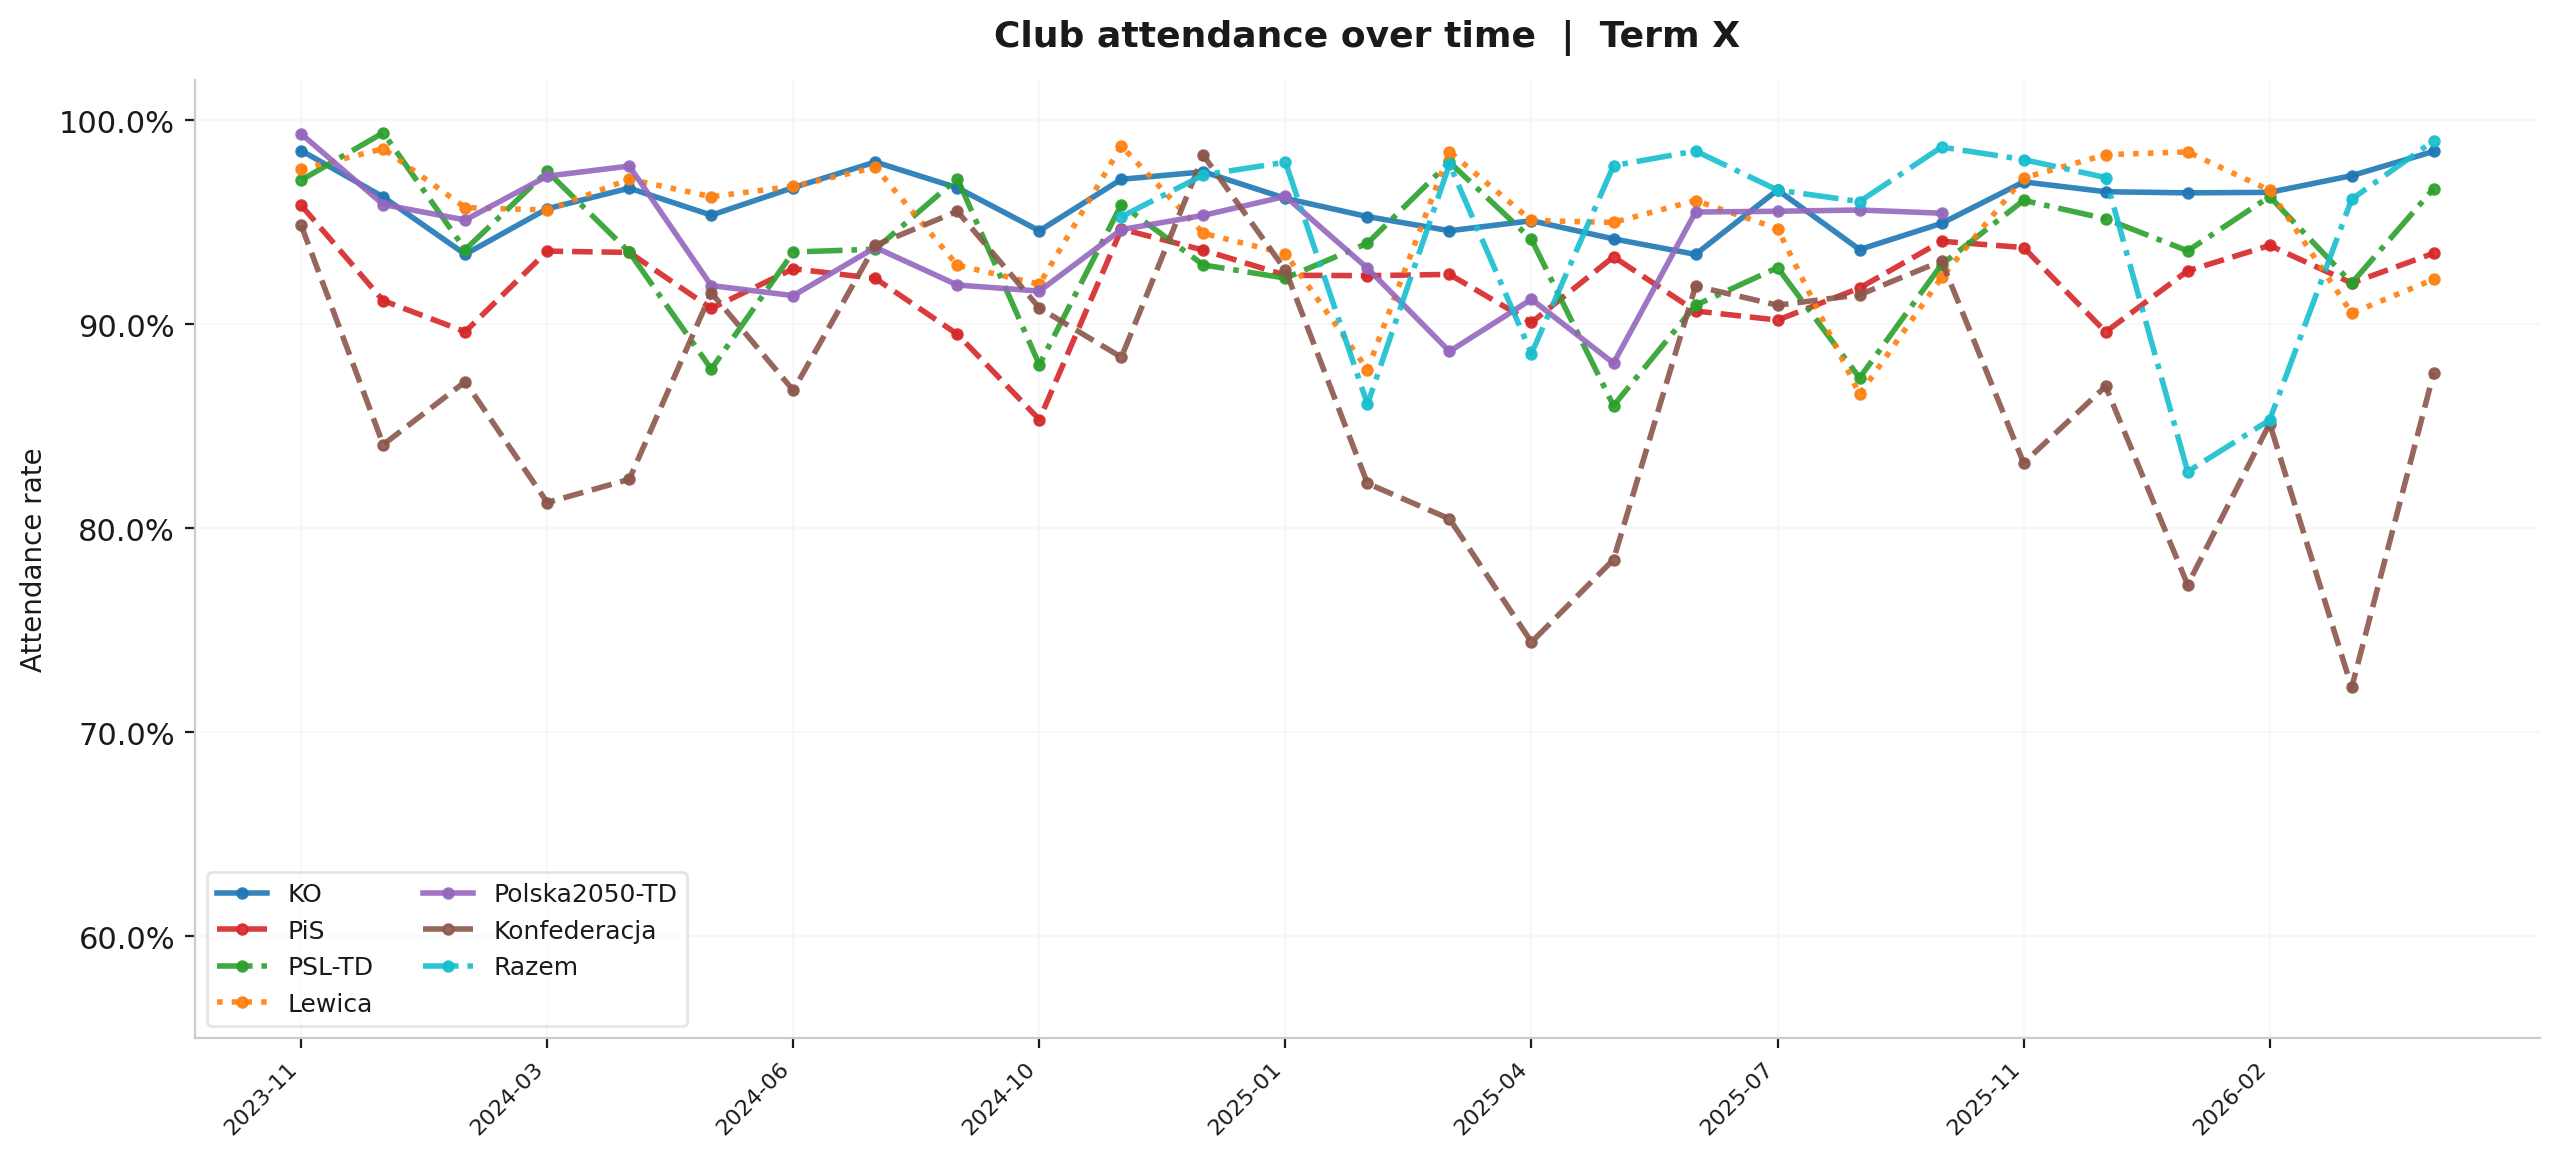
\includegraphics[width=0.95\linewidth]{fig12_attendance_over_time.png}\\[0.3cm]
        \flushleft
        \begin{itemize}
            \item \textbf{PiS Drops:} Opposition parties show the most volatile attendance — dips below 75\%.
            \item \textbf{Coalition Consistency:} Coalition clubs generally maintain attendance above 90\%.
            \item \textbf{Konfederacja:} Sharpest and most frequent attendance drops — correlating with contested legislative sessions where their vote would be decisive.
        \end{itemize}
    \end{minipage}%
}


\vspace{0.1cm}

\begin{columns}
    \column{0.5}
    \block{4. Structural Analysis: Community Detection}{
    \centering
    \textbf{Leiden Community Detection · Threshold 99\%}\\[0.2cm]
    
\includegraphics[width=0.76\linewidth]{fig1_community_betweenness_99.png}\\[0.2cm]
    \textit{Leiden community structure vs.\ official party clubs at 99\% threshold.
    Fill = community colour (majority club), border = official club, thick border = mismatch, node size = betweenness centrality.}
    \vspace{0.3cm}

    \flushleft
    \textbf{Key Findings:}
    \begin{itemize}
        \item \textbf{Near-perfect alignment:} NMI\,=\,0.971 — Leiden communities recover official clubs with 97\% accuracy from voting topology alone, with no party labels.
        \item \textbf{Two-level structure:} At 70\% threshold Leiden finds only 3 blocs (coalition acts as one entity); at 99\% it finds 8 — party sub-structure emerges only under strict ideological purity.
        \item \textbf{Bridge MPs (15 mismatches, 4.2\%):} MPs whose network community differs from their official club — likely rebel voters or recent party-switchers. See table in figure.
        \item \textbf{Main conclusion:} \textit{``Voting in the Polish Sejm is organized primarily along coalition--opposition lines; intra-bloc party distinctions emerge only at the highest agreement thresholds.''}
    \end{itemize}
}


    \column{0.5}
    \block{5. Structural Embedding: Coalition vs.\ Opposition}{
    \centering
    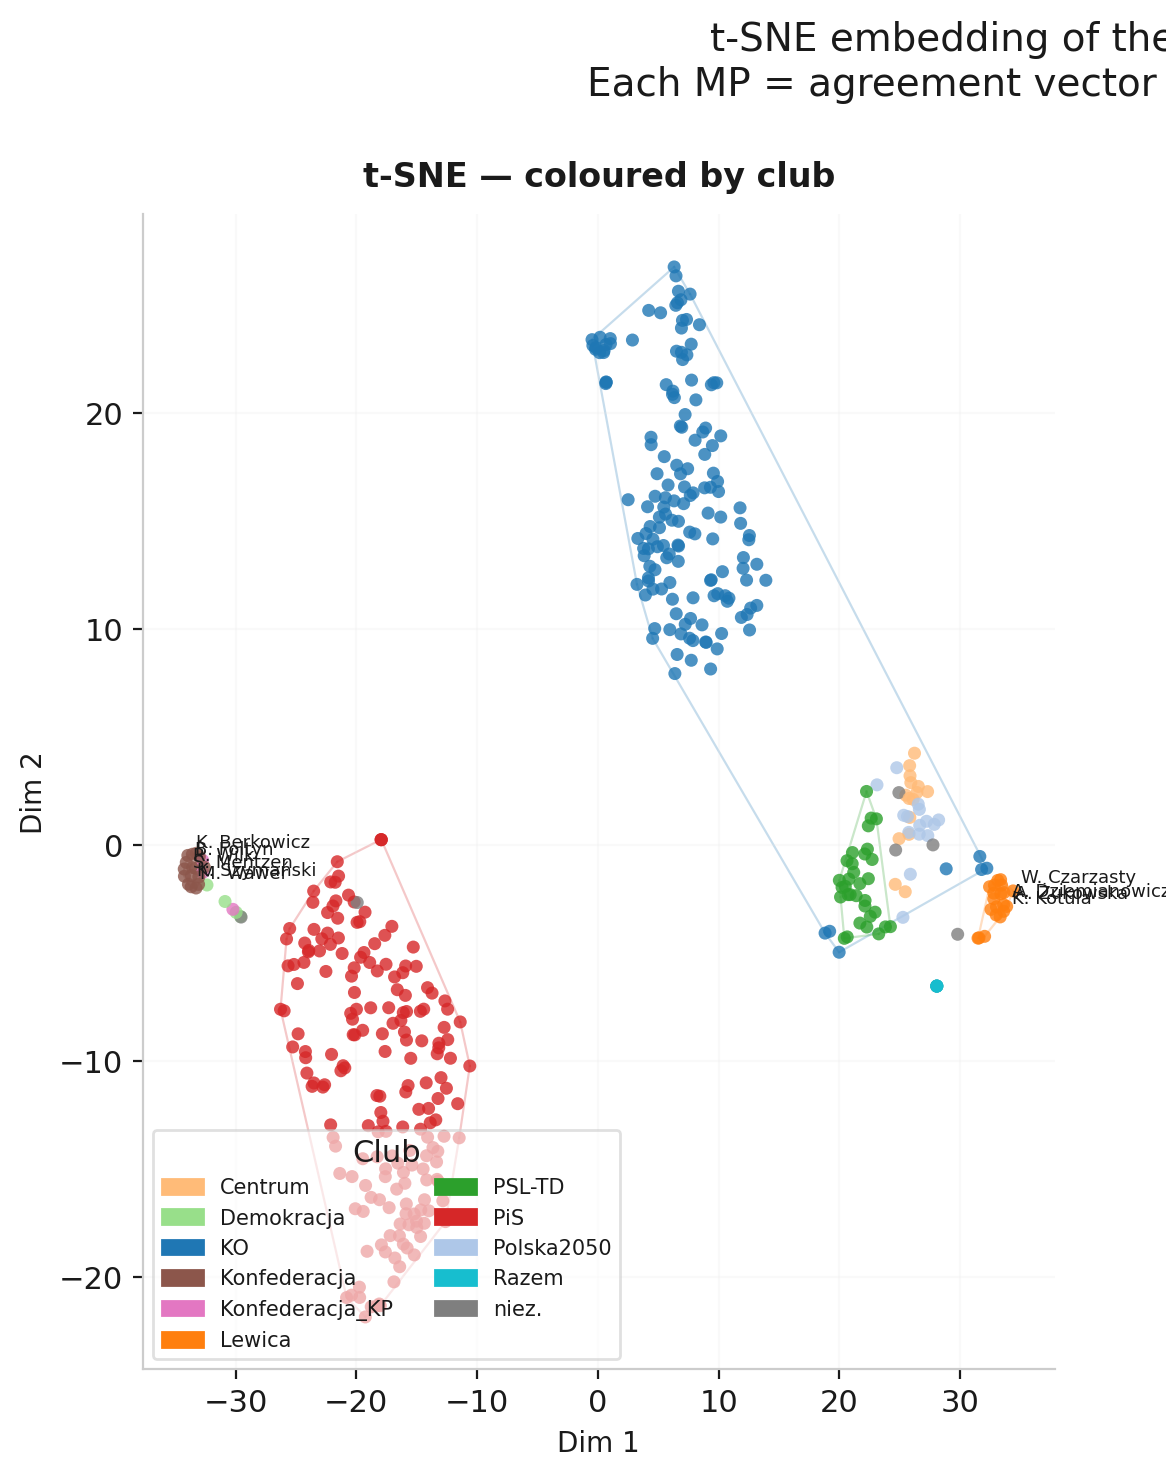
\includegraphics[height=24cm]{fig32_club_only.png}
    \vspace{0.3cm}

    \flushleft
    \textbf{Method:} t-SNE applied to the raw voting agreement vectors of all 459 MPs — \emph{no party labels used during embedding}.

    \vspace{0.4cm}
    \textbf{Key Findings:}
    \begin{itemize}
        \item \textbf{Self-organisation:} MPs cluster by party purely from voting behaviour, confirming that ideological affiliation is the dominant driver of parliamentary decisions.
        \item \textbf{Clear Divide:} Coalition (red) and opposition (dark) separate with a Silhouette score of \textbf{0.680} — a strong and statistically significant split.
        \item \textbf{Bridge MPs:} A small set of independents and \textit{Demokracja} MPs appear in the border zone, acting as potential cross-bloc mediators.
    \end{itemize}
}
\end{columns}


\end{document}